\documentclass{article}

\usepackage[utf8]{inputenc}
\usepackage{ngerman}
\usepackage{lmodern}
\usepackage{amsthm}
\usepackage{amssymb}
\usepackage{amsmath}
\usepackage[paper=a4paper,left=25mm,right=25mm,top=25mm]{geometry}
\usepackage{mathtools}
\usepackage{graphicx}
\usepackage{paralist}
\usepackage{color}

\newtheorem{satz}{Satz}
\newtheorem{definition}[satz]{Definition}
\newtheorem{lemma}[satz]{Lemma}
\newtheorem{proposition}[satz]{Proposition}
%Create a new theorem by writing \newtheorem{How to call this type of theorem}[satz]{What should be written}. Make sure to keep "satz" to ensure consecutive numeration.
% %  Variablen Definition...............
\newcommand*{\R}{k[X_{1},\ldots,X_{n}]}
\newcommand*{\indx}[2]{{#1}_{#2}}
\newcommand*{\potx}[2]{{#1}^{#2}}
\newcommand*{\N}{\mathbb{N}_0}
\newcommand*{\hf}[1]{$\prescript{a}{}{HF}_{#1}$}
\newcommand*{\hp}[1]{$\prescript{a}{}{HP}_{#1}$}
\newcommand*{\kette}[2]{$1\leq {#1}_1<{#1}_2<{#1}_3<...<{#1}_{#2}\leq n$}
\newcommand*{\dkette}[2]{${#1}_1,{#1}_2,{#1}_3,\ldots,{#1}_{#2} \in \mathbb{N}$}
\newcommand*{\Rr}[2]{$ k[X_{{#1}_{1}},\ldots,X_{{#1}_{#2}}]$}
%\newcommand*{\hf}{}
\newcommand*{\ideal}{$I$}


\title{Dimension von Varietäten}
\date{\today}
\author{Yvan Ngumeteh \and Emma Ahrens}

\begin{document}

\maketitle
%\tableofcontents

\section{Abstract}
\section{Einleitung}
	
	Sei \(S \subseteq \R\) eine Teilmenge eines Polynomrings über einem algebraisch abgeschlossenen
	Körper k. Dann ist \(V(S) := \{x \in k^n\,|\, f(x)=0\; \forall f \in S\}\) eine Varietät bzw.
	algebraische Menge. Andersherum nennt man für eine Teilmenge \(V \subseteq k^{n}\) das 
	Ideal \(I(V) := \{f \in \R\,|\, f(x)=0\; \forall x\in V\}\) das Verschwindungsideal von V.
	Mit Hilfe von Hilbert's Nullstellensatz können wir eine Bijektion von
	der Menge der Wurzelideale\footnote{Ein Wurzelideal \(\sqrt{I}\) ist ein Ideal für welches gilt: Sei \(f^{m} \in \sqrt{I}\), dann ist auch \(f \in \sqrt{I}\).} aus \(\R\) auf die Menge der Varietäten definieren. Dies gibt uns
	die Möglichkeit, unser Wissen über Ideale auf Varietäten zu übertragen. Wir haben schon
	gesehen, dass z.B. das Verschwindungsideal von Vereinigungen von Varietäten dem Schnitt der
	Verschwindungsideale der einzelnen Varietäten entspricht.
	In Abbildung~\ref{circle} und~\ref{paraboloid} sind beispielhaft zwei Varietäten dargestellt.

	\begin{figure}[ht]
		\centering
		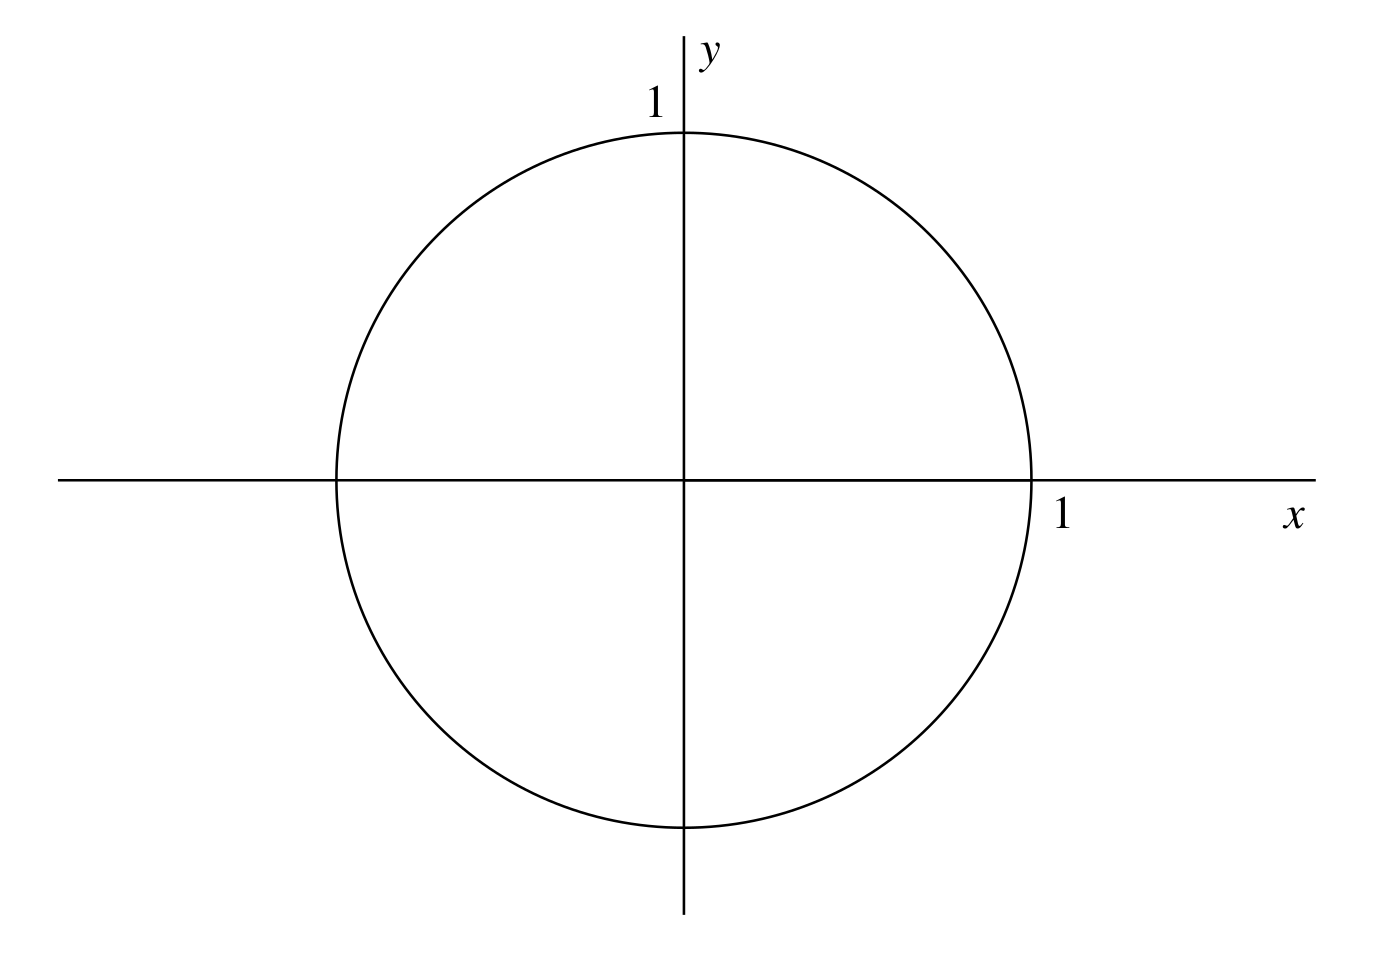
\includegraphics[width=.75\linewidth]{circle.png}
		\caption{Die Varietät \(V(X^2 + Y^2 -1)\) aus \cite{CLOS}}
		\label{circle}
	\end{figure}

	\begin{figure}[ht]
		\centering
		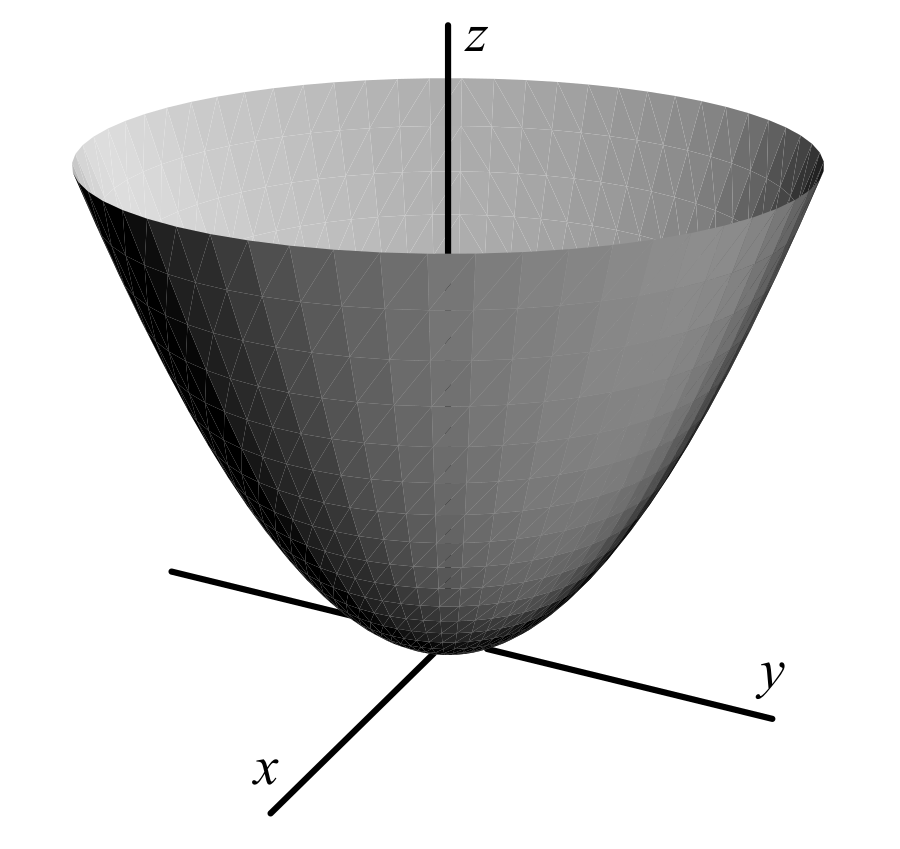
\includegraphics[width=.5\linewidth]{paraboloid.png}
		\caption{Das elliptische Paraboloid \(V(Z - X^2 -Y)\) aus \cite{CLOS}}
		\label{paraboloid}
	\end{figure}

	Im Folgenden interessieren wir uns für die Dimension einer Varietät. Intuitiv würde man
	die Varietät aus Abb.~\ref{circle} eindimensional und die aus Abb.~\ref{paraboloid}
	zweidimensional nennen. Bevor wir mit der - etwas längeren - mathematischen Definition einer
	der Dimension einer Varietät beginnen, betrachten wir zunächst einen etwas leichteren Fall 
	aus \cite{CLOS}.
	Für das Beispiel brauchen wir die Ebene \(H_x := \{(x,y,z) \in k^3\;|\; x = 0\}\) und die
	Gerade \(H_{xy} := \{(x,y,z) \in k^3\;|\; x=0 \wedge y=0\}\).

	Überlegen wir uns nun die Dimension von der Varietät des Monomialideals
	\(I := (Y^2Z^3, X^5Z^4, X^2YZ^2)\) in \(k[X,Y,Z]\). Dann wissen wir
	\begin{align*}
		V(I) &= V(Y^2Z^3, X^5Z^4, X^2YZ^2) \\
		&= V(Y^2Z^3) \cap V(X^5Z^4) \cap V(X^2YZ^2) \\
		&= (H_y \cup H_z) \cap (H_x \cup H_z) \cap (H_x \cup H_y \cup H_z) \\
		&= H_z \cup (H_y \cap H_x \cap (H_x \cup H_y))
	\end{align*}
	Der Schnitt der zwei Ebenen \(H_x\) und \(H_y\) ist die Gerade \(H_{xy}\) und
	\(H_{xy} \cap (H_x \cup H_y) = H_{xy}\), also folgt
	\begin{displaymath}
		V(I) = H_z \cup H_{xy}.
	\end{displaymath}
	Die Varietät besteht also aus der xy-Ebene und einer Geraden, die darauf senkrecht steht.
	Es gibt also einen Teil, der intuitiv eindimensional erscheint und einen zweidimensionalen.
	Später werden wir sehen, dass die Dimension einer Varietät die maximale Dimension der einzelnen
	Teile der Varietät ist - für das Beispiel ist sie also 2.
	
	\colorbox{yellow}{
	Ganz am Ende nochmal auf Kreis und Paraboloid eingehen!
	Geschichtliches. Warum will man überhaupt etwas über die Dimension von Varietäten wissen.
	Wo könnte das nützlich sein?}

\section{Dimension von Monomidealen}
	
	Wir beginnen damit, für ein Ideal \(I\) eine möglichst einfache k-Basis von \(\R/I\) zu finden.
	Damit der Beweis unseres ersten Satzes nicht zu lang wird, müssen wir allerdings noch ein
	bisschen Vorarbeit leisten.

	\begin{lemma} \label{1.2.3}
	Sei \(I \subseteq \R\) ein Ideal, das von einer Menge G von Monomen erzeugt wird. Dann liegt
	ein Polynom \(f \in \R\) in I genau dann, wenn für jeden Term \(a_{j}X^{\alpha_{j}}\) von f ein
	\(g \in G\) existiert, welches \(a_{j}X^{\alpha_{j}}\) teilt.
	\end{lemma}

	\begin{proof}[Beweis]
	Sei \(f \in I\). Dann gilt \(f = \sum_{i=1}^{s} h_{i}g_{i}\) mit \(h_{i} \in R\) und \(g_{i}
	\in G\). Damit hat jeder Term die Form \(h_{i}g_{i}\) und ist somit durch ein Element aus G
	teilbar.
	Sei nun andersherum \(f \in \R\) und für jeden Term \(a_{j}X^{\alpha_{j}}\) von f existiert ein
	\(g \in G\), welches \(a_{j}X^{\alpha_{j}}\) teilt. Dann kann man f als Linearkombination von 
	Elementen aus G schreiben und damit liegt f nach der Definition eines Ideals in I.
	\end{proof}


	\begin{lemma} \label{1.2.4}
	Sei \((g_{i})_{i \geq 1}\) eine Folge von Monomen in \(\R\) mit \(g_{1} \succeq g_{2} \succeq
	\ldots\) für eine Monomialordnung \(\preceq\). Dann existiert ein \(r \in \mathbb{N}\) mit 
	\(g_{n} = g_{r}\) für alle \(n \geq r\). 
	\end{lemma}

	\begin{proof}[Beweis]
	Sei \(I = ((g_{i})_{i \geq 1})\), dann ist I ein Ideal. Nach dem Hilbert'schen Basissatz
	wissen wir, dass I endlich erzeugt ist. Also existiert ein r, so dass die Menge \(G = \{g_{1},
	\ldots, g_{r}\}\) I erzeugt. Für ein \(i \geq r\) und \(g_{i} \in I\) existiert ein
	\(j \in \underline{r}\), so dass \(g_{j}\; | \;(g_{i}\) nach Lemma~\ref{1.2.3}. Also \(g_{i}
	\succeq g_{j} \succeq g_{r}\). Andererseits gilt nach Voraussetzung, dass \(g_{i} \preceq g_{r}
	\), also folgt \(g_{i} = g_{r}\).
	\end{proof}

	Lemma~\ref{1.2.4} sagt uns insbesondere, dass in jeder abzählbaren Menge von Mnomen ein
	kleinstes Element existiert.
	

	\begin{proposition}[Divisionsalgorithmus] \label{1.2.5}
	Sei \(\preceq\) eine Monomialordnung und \(f, f_{1}, \ldots, f_{s} \in \R\) nicht null. Dann
	gilt \begin{displaymath} f = \sum_{i=1}^{s} h_{i}f_{i}\; + r, \end{displaymath} mit
	\(r, h_{1}, \ldots, h_{s} \in \R\) und \(LT(h_{i}f_{i} \preceq LT(f)\) für alle \(h_{i} \neq 0
	\) und \(r = 0\) oder kein Term von r wird durch ein \(LT(f_{i})\) geteilt für \(i \in
	\underline{s}\).
	\end{proposition}

	\begin{proof}[Beweis]
	Wir beweisen diese Proposition per \colorbox{yellow}{Rückwärtsinduktion über LT(f) beginnend mit dem größten Term.} \\
	Beim Induktionsschritt unterscheiden wir drei Fälle:\\
	Sei f konstant, dann gilt \(f = \sum_{i=1}^{s} 0f_{i}\; + r\) mit \(r := f\) und \(h_{i} := 0\). \\
	Falls ein \(i \in \underline{s}\) existiert, so dass \(LT(f_{i})\;| \; LT(f)\), setzen wir
	\begin{displaymath} f^{(1)} := f - \frac{LT(f)}{LT(f_{i})}f_{i}.\end{displaymath} Dann gilt
	\( f = f^{(1)} + \frac{LT(f)}{LT(f_{i})}f_{i} \) mit \(h_{i} = \frac{LT(f)}{LT(f_{i})}\) und 
	\(LT(h_{i}f_{i}) = LT(f) \preceq LT(f).\) \\
	Falls kein solches \(f_{i}\) existiert, schreiben wir \begin{displaymath} f^{(1)} := f -
	LT(f). \end{displaymath} Und \(f = f^{(1)} + LT(f)\) mit \(r = LT(f)\) erfüllt die Bedingungen 
	(insbesondere, dass kein Term von r durch ein \(LT(f_{i})\) geteilt wird). \\
	Führe den Schritt nun induktiv auf \(f^{(1)}\) durch bis \(f^{(j)} = 0\) und bestimme
	\(h_{1}, \ldots, h_{s}, r\) durch Rückwärtseinsetzen.
	\end{proof}


	Jetzt kommen wir zu dem ersten Satz, der direkt für die Dimension von Varietäten wichtig ist.


	\begin{satz} \label{1.2.8}
	Sei \(\{0\} \neq I \subseteq \R\) ein Ideal und \(\preceq\) eine Monomialordnung auf
	\(\mathbb{N}^{n}_{0}\). Sei G eine Gröbnerbasis von I mit I = (G). Dann ist eine k-Basis von 
	\(\R/I\) gegeben durch die Restklassen von \(X^{\alpha}\) mit
	\begin{displaymath}
	\alpha \in C(I) := \{\alpha \in \mathbb{N}^{n}_{0}\; |\;\; LT(g) \nmid X^{\alpha}\; \forall g 
	\in G\}.
	\end{displaymath}
	\end{satz}

	\begin{proof}[Beweis]
	Wir zeigen erst, dass die Monome mit Exponent aus C(I) ganz \(k[X_{1},\ldots,X_{n}]/I\) 
	aufspannen und anschließend, dass kein Element aus I durch echte Linearkombination solcher
	Monome dargestellt werden kann. \\
	Sei \(G = \{f_{1}, \ldots, f_{s}\}\) und \(0 \neq f \in \R\). Dann ist
	\(f = \sum_{i=1}^{s} h_{i}f_{i}\; + r = f' + r\) nach Proposition~\ref{1.2.5} mit \(r=0\) oder 
	\(r = a_{l}X^{\alpha_{l}} + \ldots + a_{0}\) mit \(LT(f_{i}) \nmid X^{\alpha_{j}}\) 
	für jedes \(i \in \underline{s}\) und \(j \in \underline{l}\). Also ist \(r\) eine
	Linearkombination von Monomen \(X^{\alpha_{j}}\) mit \(\alpha_{j} \in C(I)\).
	Es gilt außerdem \([f] = [r]\) in \(\R/(G)\) und damit erzeugen die
	Monome mit \(\alpha \in C(I)\) den ganzen Restklassenring. \\
	Angenommen es existiert \(f = f' + r \in I\) mit \(r \neq 0\) und f' und r wie oben.
	Dann gilt \(0 \neq r = f - f'\). Da \(f \in I\) und \(f' \in I\) folgt
	\(r \in I\), womit folgt, dass \((LT(r) \in (LT(f_{1}), \ldots, LT(f_{s}))\).
	Nach Lemma~\ref{1.2.3} existiert dann ein \(f_{i}\) mit \(LT(f_{i})\; |\; LT(r)\). Dies ist 
	ein Widerspruch, also folgt \(r = 0\) und die Restklassen von \(X^{\alpha}\) mit
	\(\alpha \in C(I)\) sind linear unabhängig in \(\R/I\).
	\end{proof}
	
	
	In Abb.~\ref{dots} sieht man ein Koordinatensystem von \(\mathbb{N}^{2}_{0}\). Jeder Punkt
	\(\alpha\) repräsentiert dabei ein Monom \(X^{\alpha}\) für welches gilt \(X^{\alpha} = LM(f)\)
	für ein \(f \in \R\). Die Punkte in dem grau hinterlegten Teil stehen nun für die Monome, die
	Elemente aus \(LM(I)\) sind. Die unausgefüllten Punkte stehen für Monome aus C(I).

	\begin{figure}[ht]
		\centering
		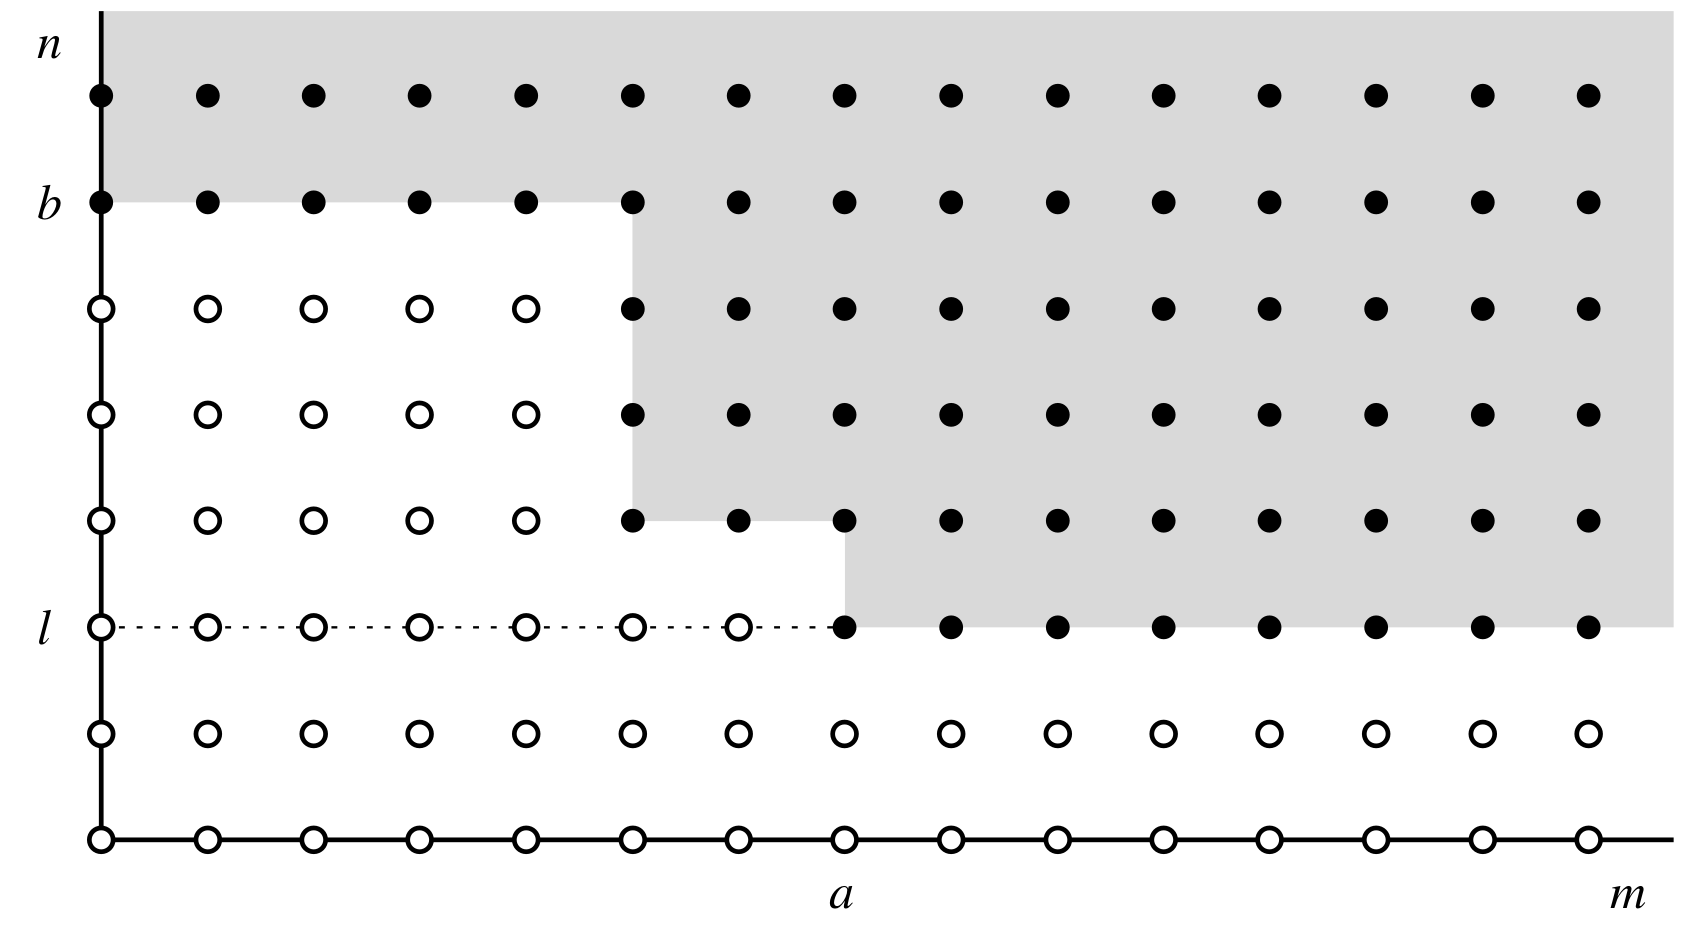
\includegraphics[width=.75\linewidth]{Dots.png}
		\caption{Anschauliche Darstellung von \(\R/I\) aus \cite{CLOS}}
		\label{dots}
	\end{figure}


	\begin{definition} \label{1.2.11}
	Sei \(I \subseteq \R\) ein Ideal und \(s \in \mathbb{N}_{0}\). Dann definiere \(I_{\leq s} :=
	I \cap \R_{\leq s}\). Nun gilt, dass \(\R_{\leq s}\) ein endlich dimensionaler Vektorraum über
	k  mit \(I_{\leq s}\) als Teilraum ist. Wir können die Funktion \begin{displaymath}
	\prescript{a}{}{HF}_{I} : \mathbb{N}_{0} \rightarrow \mathbb{N}_{0}, \quad s \mapsto
	dim_{k}(\R_{\leq s}/I_{\leq s})	\end{displaymath} definieren, die (affine) Hilbertfunktion
	von I genannt wird.
	\end{definition}

	
	\begin{lemma}
	Es gilt \(|M_{n,s}| := |\{\alpha \in \mathbb{N}^{n}_{0}\; |\; |\alpha| \leq s \}| = \binom{s + n}{s}. \)
	\end{lemma}

	\begin{proof}[Beweis]
	Induktionsanfang: Sei \(n = 2\), \(s \in \mathbb{N}\) fest und \(\alpha = (\alpha_{1}, 
	\alpha_{2}) \in \mathbb{N}^{2}_{0}\). Wähle \(\alpha_{1} \in \{0, \ldots, s\}\). Dann muss
	\(\alpha_{2} \in \{0, \ldots, s - \alpha_{1}\}\) gelten, damit \(|\alpha| = \alpha_{1} +
	\alpha_{2} \leq s\). Nun wissen wir, dass
	\begin{align*}
		|M_{2,s}| &= \sum_{i=0}^{s} s-i+1 = s(s+1) - \frac{s(s+1)}{2} + (s+1) \\
		&= (s+1)(s - \frac{s}{2} + 1) = (s+1)(2s - s +2)\frac{1}{2} \\
		&= (s+1)(s+2)\frac{1}{2} = \frac{(s+1)!}{2!\,s!} = \binom{s+2}{s}
	\end{align*}
	
	Induktionsvoraussetzung: Die Behauptung gelte für ein \(n \in \mathbb{N}_{\geq 2}\).

	Induktionsschritt: Sei \(n \in \mathbb{N}_{\geq 2}\) mit \(|M_{n,s}| = \binom{s + n}{s}\). Wir
	betrachten \(\alpha \in \mathbb{N}^{n+1}_{0}\) und können \(\alpha\) auch schreiben als
	\(\alpha = (\beta, \alpha_{n+1})\) mit \(\beta \in \mathbb{N}^{n}_{0}\). Sei \(\alpha_{n+1}
	\in \{0, \ldots, s\}\), dann muss \(\beta \in M_{n,s-\alpha_{n+1}}\) sein, damit
	\(|\alpha| \leq s\). Also folgt mit der Induktionsvoraussetzung und einer Indexverschiebung
	\begin{align*}
		|M_{n+1,s}| &= \sum_{i=0}^{s} |M_{n,s-i}| = \sum_{i=0}^{s} \binom{s-i+n}{s-i} \\
		&= \sum_{i=0}^{s} \binom{i+n}{i} = \binom{s+(n+1)}{s}
	\end{align*}

	Damit folgt die Behauptung nach dem Induktionsprinzip.
	\end{proof}

	\paragraph{Ein paar Beispiele}
	\begin{itemize}
	\item Sei \(I = \R\). Dann ist
		\begin{align*}
			\prescript{a}{}{HF}_{I}(s) &= dim_{k}(\R_{\leq s}/I_{\leq s}) \\
			&= dim_{k}(\R_{\leq s}/\R_{\leq s}) \\
			&= dim_{k}(\emptyset) \\
			&= 0
		\end{align*}
	 für alle \(s \in \mathbb{N}_{0}\).  
	\item Sei nun \(I = \{0\}\). Dann ist mit Satz~\ref{1.2.8} und dem Theorem aus der Kombinatorik
		\begin{align*}
			\prescript{a}{}{HF}_{I}(s) &= dim_{k}(\R_{\leq s}/I_{\leq s}) \\
			&= dim_{k}(\R_{\leq s}) \\
			&= |\{ X^{\alpha} \in \R\, |\; deg(X^{\alpha}) \leq s\}| \\
			&= |\{ \alpha \in \mathbb{N}^{n}_{0}\, |\; |\alpha| \leq s\}| = |M_{n,s}| \\
			&= \binom{s+n}{s} = \binom{s+n}{n} \\
			&= \frac{1}{n!}(s+n)(s+n-1)\cdots (s+1) \\
			&= \frac{1}{n!}s^{n} + \frac{1}{n!}\binom{n+1}{2}s^{n-1} + \cdots + 1. \\
		\end{align*}
	\item Gehen wir noch einmal kurz zu Abb.~\ref{dots} zurück. Hier ist betrachten wir ein 
	Ideal I aus \(k[X,Y]\). Es gilt \(\prescript{a}{}{HF}_{I}(6) = 36\),
	\(\prescript{a}{}{HF}_{I}(8) = 40\) und \(\prescript{a}{}{HF}_{I}(9) = 42\).
	Für \(s \geq 7\) gilt \(\prescript{a}{}{HF}_{I}(s+1) = \prescript{a}{}{HF}_{I}(s) + 2\),
	die Funktion wächst also linear. Man kann die Hilbertfunktion sogar direkt an der Abbildung
	ablesen: Für \(s \geq 7\) gilt \(\prescript{a}{}{HF}_{I}(s) = 2*s + 22\).
	\end{itemize}

	Überlegen wir uns kurz den Zusammenhang zwischen der \glqq gefühlten\grqq  Dimension einer Varietät und
	dem Grad der Hilbertfunktion. Im ersten Beispiel ist \(V(I) = \{0\}\) und die gefühlte
	Dimension ist 0. Dies entspricht auch dem Grad der Hilbertfunktion. Im zweiten Beispiel ist
	\(V(I) = k^n\) mit Dimension n und auch die Hilbertfunktion hat den Grad n. Für die Varietät 
	aus Abb.~\ref{dots} gilt \(V(I) = \{(x,y) \in k^2\;|\; y = 0\} = H_y\). Also ist \(V(I)\)
	intuitiv eindimensional, was ebenfalls dem Grad der Hilbertfunktion entspricht.

	Diese Vermutungen wollen wir jetzt beweisen.

	\begin{lemma}[Macaulay] \label{1.2.13}
	Sei \(\preceq\) eine gradierte lexikographische Monomialordnung und \(I \subseteq \R\) ein
	Ideal. Dann ist \(\prescript{a}{}{HF}_{I}(s) = \prescript{a}{}{HF}_{LT(I)}(s)\) für alle
	\(s \in \mathbb{N}_{0}\).
	\end{lemma}

	
	\begin{proof}[Beweis]
	Zunächst definieren wir uns die Menge
	\begin{displaymath}
		D := \{ LM(f) \; | \; 0 \neq f \in I \} = \{LM(f_1), \ldots, LM(f_m)\}
	\end{displaymath}
	für ein \(m \in \mathbb{N}_{0}\) und \(f_{i} \in I\) für alle \(i \in \underline{m}\). Die
	zweite Gleichheit gilt aufgrund der Endlichkeit von \(I\).
	Wir betrachten außerdem die Menge
	\begin{displaymath} B := \{f_{1}, \ldots, f_{m}\}. \end{displaymath}
	Die Elemente aus B entsprechen denen aus der Menge D.

	Wir zeigen nun, dass D eine k-Basis von \((LT(I))_{\leq s}\) und B eine k-Basis von \(I\) ist.
	Dann folgt nämlich, dass die beiden Mengen die selbe Kardinalität und die erzeugten
	Vektorräume die selbe Dimension haben, womit das Lemma von Macaulay gezeigt ist.

	Als Erstes wollen wir zeigen, dass D eine k-Basis von \((LT(I))_{\leq s}\) ist. Da D die
	Leitmonome der Elemente aus I enthält, ist D offensichtlich linear unabhängig.
	Wir zeigen also, dass das Erzeugnis von D ganz \((LT(I))_{\leq s}\) aufspannt: Dazu
	betrachten wir ein beliebiges \(g \in (LT(I))_{\leq s}\). Es gilt \(deg(g) \leq s\) und da D
	alle \(LT(I)\) mit Grad \(\leq s\) enthält, kann man schreiben 
	\(g = \sum_{i=1}^{m} h_{i}LT(f_{i})\) mit \(h_{i} \in k\) für alle \(i \in \underline{m}\).
	Also ist \(g \in (D)\) und damit spannt D ganz \((LT(I))_{\leq s}\) auf. Es folgt also, dass
	D eine k-Basis von \((LT(I))_{\leq s}\) ist.
	
	Jetzt zeigen wir, dass B eine k-Basis von \(I\) ist. Die lineare Unabhängigkeit der einzelnen 
	Elemente können wir durch einen einfachen Widerspruchsbeweis zeigen:
	Sei \(0 = \sum_{i=1}^{m} h_{i}f_{i}\), \(h_{i} \in k\) für alle \(i \in \underline{m}\),
	und es existiert ein \(i \in \underline{m}\) mit \(h_{i} \neq 0\).
	Da \(f_{i} \neq 0\) ist, existiert mindestens ein \(i \neq j \in \underline
	{m}\) mit \(h_{j} \neq 0\). Ohne Beschränkung der Allgemeinheit kann man annehmen, dass genau
	zwei Koeffizienten \(\neq 0\) existieren. Dann gilt
	\begin{align*}
		0 &= \sum_{i=1}^{m} h_{i}f_{i} = h_{i}f_{i} + h_{j}f_{j} \\
		&\Leftrightarrow -h_{j}f_{j} = h_{i}f_{i} \\
		&\Leftrightarrow -\frac{h_{j}}{h_{i}} f_{j} = f_{i}.
	\end{align*}
	Also gilt \(LM(f_{j}) = LM(f_{i})\), dies ist aber ein Widerspruch zur Definition der Menge B,
	also ist B linear unabhängig. \\
	Wir wählen nun ein \(g \in I\). Dann existiert ein \(i \in \underline{m}\) mit \(LM(f) =
	LM(f_{i})\), weil \(f \in I\), also auch \(LM(f) \in D\). Wir definieren
	\begin{align*}
		f^{(1)} := f - \frac{LM(f)}{LM(f_{i})}f_{i} \\
		\Leftrightarrow f = f^{(1)} + \frac{LM(f)}{LM(f_{i})}f_{i}.
	\end{align*}
	Es gilt \(LM(f) = LM(\frac{LM(f)}{LM(f_{i})}f_{i})\), also folgt \(LM(f^{(1)}) \preceq LM(f)\),
	da wir die Monome unter gradierter lexikographischer Ordnung betrachten.
	Für \(f^{(1)}\) existiert wie für f wieder ein \(j \in \underline{m}\) mit \(LM(f) =
	LM(f_{j})\), da \(f^{(1)} \in I\). Wir definieren \(f^{(2)}\) analog zu oben und es
	folgt \(LM(f^{(2)}) \preceq LM(f^{(1)})\). Das machen wir induktiv weiter bis \(f^{(l)} = 0\)  
	für ein \(l \in \mathbb{N}\).
	Der Algorithmus endet nach endlich vielen Iterationen, da \(LM(f) \succeq LM(f^{(1)}) \succeq LM(f^{(2)}) \succeq \cdots\).
	Also kann man g als k-Linearkombination von Elementen aus B schreiben, damit spannt B ganz \(I\) und B ist eine Basis von \(I\).
	\end{proof}

	
	\colorbox{yellow}{Was wir bis jetzt wissen}


\section{Dimension von beliebigen Idealen}

\subsection{Das Hilbert-Polynom}

Im folgenden sei $n \in \mathrm{N}$ beliebig aber fest.

\begin{satz}
	\label{1.2.14}
	Sei  \ideal $\unlhd$ $\R$, dann existiert ein eindeutiges Polynom \hp{I}(t) $\in \mathbb{Q}[t]$ (t ist eine Variable) und $\indx{s}{0}\geq0$,  sodass \hp{I}(s)=\hf{I}(s)= $\indx{dim}{k}$ ($\indx{\R}{\leq s}$/$\indx{I}{\leq s}$), für alle $ s\geq\indx{s}{0}$. Weiterhin besitzt \hp{I}(t) folgende Eigenschaften:	
\end{satz}
\begin{compactenum}
	\item[a)] Der Grad von \hp{I}(t) ist der größte $d \in \mathbb{N}$, sodass es \dkette{i}{d} mit \kette{i}{d} existieren und $I\cap k[X_{{i}_{1}},\ldots,X_{{i}_{d}}]={\emptyset}$.
	\item[b)] Sei $d=grad(\textnormal{\hp{I}})$. Dann gilt \hp{I}(t)=$\sum_{k=0}^{d} \indx{a}{k}t^k$ mit $\indx{a}{k}d! \in \mathbb{Z}, \forall k\in \underline{\indx{d}{0}}$ und $\indx{a}{d}d!>0$
\end{compactenum}

\begin{proof}[Beweis]
	Wir bemerken, dass \hp{I}(t) sobald existent eindeutig ist, da es ein Polynom ist. Es muss also nur die Existenz nachgewiesen werden. Im Folgenden ist $s\in \N$ beliebig aber fest gewählt, falls nicht anders spezifiziert wird.\\
	
	Für die trivialen Fälle $I=(0)$ gilt, wegen \hf{I}(s)= $\indx{dim}{k}$ ($\indx{\R}{\leq s}$/$\indx{I}{\leq s}$)$=$ $\left|M\right|=\binom{n+s}{s}, \forall s\in \N$.
	
	Oder $I=\R$,wegen \hf{I}(s)= $\indx{dim}{k}$ ($\indx{\R}{\leq s}$/$\indx{I}{\leq s}$)$=0, \forall s\in \N$  (also \hp{I}$=0$ ist das Nullpolynom !) die Behauptungen.
	
	
	Wir gehen im Folgenden in fünf Schritten vor.\\
	\begin{compactenum}
		
		\item Nehmen wir also an, dass $I$ nicht trivial ist. Sei $G$ eine Gröbner-Basis von $I$ (bzgl. eine graduierte lexikographische Ordnung) und $M=\{\alpha \in \N^n:\exists\;f\in G \textnormal{ sodass } LM(f)=\potx{X}{\alpha}\}$
		\begin{displaymath}
		\{LM(g):g\in G\}=\{\potx{X}{\beta}:\beta \in M \}
		\end{displaymath}
		
		 Die Mächtigkeit von $M$ ist endlich , da nach dem Hilbert'sche Basissatz $G$ eine endliche Menge von Mononen ist.
		Wir setzen im Folgenden 
		\begin{displaymath}
		C(I):=\{\alpha \in \N: \potx{X}{\beta} \nmid \potx{X}{\alpha},\; \forall \beta \in M \}
		\textnormal{ und } 
		\indx{C(I)}{\leq s}:= \{\alpha \in \N:|\alpha|\leq s, \; \potx{X}{\beta} \nmid \potx{X}{\alpha},\; \forall \beta \in M \}
		\end{displaymath}
		
Behauptung: $\forall s\geq 0$ gilt \hf{I}(s)$=|\indx{C(I)}{\leq s}|$.\\

\begin{proof}[Beweis]
Nach Macaulay() gilt \hf{I}(s)=\hf{(LT(I))}(s), für alle $ \in s\geq0$. Das heißt,
\begin{displaymath}
\indx{dim}{k} (\indx{\R}{\leq s}/\indx{I}{\leq s})=\indx{dim}{k}(\indx{\R}{\leq s}/\indx{(LT(I))}{\leq s}).
\end{displaymath}

Weiterhin gilt mit Definition (1.2.7)(Buchberger), dass $H=\{\potx{X}{\beta}:\beta \in M \}$ eine Gröebner-Basis von (LT(I)) ist. Mit Satz \ref{1.2.8} bilden die Restklassen von $\potx{X}{\alpha}$ ($\alpha\in C(I)$) eine $k$-Vektorraum-Basis von $\R/(LT(I))$. Daraus folgt die Behauptung.\\
\end{proof}
\item Seien $J\subseteq \underline{n}$ und eine Abbildung $\tau:J\longrightarrow \N$ gegeben. Wir definieren
\begin{displaymath}
C(J,\tau):=\{\alpha \in (\N)^n: \indx{\alpha}{j}=\tau(j), \forall \in J  \}
\end{displaymath}

Behauptung: Es existiert eine endliche Menge $\chi$ von Tupeln (J,$\tau$), sodass 

\begin{displaymath}
(\star)\;\;\;   C(I)=\bigcup\limits_{(J,\tau)\in \chi} C(J,\tau)  
 \end{displaymath}

\begin{proof}[Beweis]
	Für $\beta:=(\indx{\beta}{1},\ldots,\indx{\beta}{n}) \in \N$, definiert man 
	
	\begin{displaymath}
	C(\beta):=\{\alpha\in \potx{\N}{n}: \potx{X}{\beta}\nmid\potx{X}{\alpha}\}
	\end{displaymath}
	Dann gilt $C(I)=\bigcap\limits_{\beta\in M}C(\beta)$. 
	Weiterhin gilt falls $(J,\tau),(J\prime,\tau\prime)$ zwei Tupeln, wie oben definiert sind
	
	\begin{displaymath}
	(\star \star)\;\;\;   C(J,\tau)\cap C(J\prime,\tau\prime)=\left\{\begin{array}{ll} \emptyset & ,falls  \;\tau(j)\neq\tau\prime(j)\; \textnormal{ für einige } j\in J\cap J\prime \\
	\\
	C(J\cup J\prime, \tau_0) & ,sonst \end{array}\right.
	\end{displaymath} 
	wobei $\indx{\tau}{0}:J\cup J\prime \longrightarrow \N$, $ j\mapsto \tau_{0}(j)=\left\{\begin{array}{ll} \tau(j), & falls\;  j \in J \\
	\\
	\tau\prime(j), & falls\;  j \in J\prime \\
	\\
	0, & sonst \end{array}\right.$.
	
%	Also man kann O.B.d.A annehmen, dass in ($\star$) nur disjunkte $C(J,\tau)$ vereinigt werden. D.h.
%	
%	\begin{displaymath}
%	C(I)=\sum\limits_{(J,\tau)\in \chi}C(J,\tau)
%	\end{displaymath}
	Aber es gilt $\alpha \in C(\beta)\Leftrightarrow \indx{\alpha}{i}<\indx{\beta}{i}$ für einige $i\in\underline{n}$. Also gilt,
 	

 	\begin{align*}
 	C(\beta)&=\bigcup\limits_{i=1}^{n}\bigcup\limits_{t_{i}=1}^{\indx{\beta}{i}-1}\{\alpha\in \potx{\N}{n}:\indx{a}{i}=\indx{t}{i}\}\\&
 	=\bigcup\limits_{i=1}^{n}\bigcup\limits_{t_{i}=1}^{\indx{\beta}{i}-1} C({i},\tau:i\mapsto \indx{t}{i})
 	\end{align*}
 	Da $\left|M\right|$ endlich und die $C(\beta)$ jeweils endliche Vereinigungen von Mengen von Typ $C(J,\tau)$ ist, folgt die Behauptung aus ($\star \star$).\\
\end{proof}
\item Behauptung: Für alle $(J,\tau)$ im 2.Fall, existiert ein eindeutiges Polynom $\indx{F}{J,\tau}(s)\in \mathbb{Q}[t]$ mit $grad(\indx{F}{J,\tau})=n-|J|$ und
$\indx{F}{J,\tau}(s)=\left|\indx{C(J,\tau)}{\leq s}\right|$, für alle $s\geq |\tau|:=\sum\limits_{j\in J}\tau(j)$\\

\begin{proof}[Beweis]
	Sei $\gamma=(\indx{\gamma}{1},\ldots,\indx{\gamma}{n}) \in \N$, sodass $\indx{\gamma}{j}=0$, falls $j\notin J$ und $\indx{\gamma}{j}=\tau(j)$, falls $j\in J$. Dann gilt $C(J,\tau)$ ist die Menge von $\alpha+\gamma$, wo  $\alpha=(\indx{\alpha}{1},\ldots,\indx{\alpha}{n}) \in \potx{\N}{n}$ ist, sodass $\indx{\alpha}{j}=0, \forall j \in J$. Daraus folgt, dass $\left|\indx{C(J,\tau)}{\leq s}\right|$ die Anzahl von Monomen in den Variablen $\indx{X}{j}$ $(j\notin J)$, sodass multipliziert mit $\potx{X}{\gamma}$, der Grad maximal $s$ beträgt.
	
	Dies wiederum entspricht der Anzahl von Monomen in $d:=n-\left|J\right|$ Variablen deren höchstens Grad $s-\left|\gamma\right|$ beträgt, da die Variablen mit Indizes in $J$ eine durch $\tau$ vorgegebene Potenz haben und der Grad des gesamten Produkts nach oben durch $s$ beschränkt ist. Wichtig hierbei zu beachten ist, dass $\left|\gamma\right|=\left|\tau\right|$ gilt. Deswegen gilt,
	
	\begin{align*}
	\left|\indx{C(J,\tau)}{\leq s}\right|&=\binom{n-\left|J\right|+s-\left|\gamma\right|}{s-\left|\gamma\right|}=\binom{d+s-\left|\gamma\right|}{s-\left|\gamma\right|}\\&
	=\binom{d+s-\left|\gamma\right|}{d}=\frac{(d+s-\left|\gamma\right|)(d+s-\left|\gamma-1\right|\ldots(s-\left|\gamma+1\right|))}{d!}\\&
	=\frac{s^d+O(s)}{d!}=:\indx{F}{J,\tau}(s)
	\end{align*}
	,wobei $grad(O(s))<d$ gilt.	Da die Koeffizienten des obigen Polynoms eindeutig durch $d$  und $|\gamma|$ festgelegt sind, folgt die Eindeutigkeit von $\indx{F}{J,\tau}$. Hierbei hat der Leitkoeffizient von $\indx{F}{J,\tau}$ die Form $\frac{1}{d!}>0$.
\end{proof}

\item Sei $m\in\N$ beliebig aber fest vorgegeben. Falls $\indx{A}{1},\ldots,\indx{A}{m}$ endliche Teilmengen von einer Menge $T$ sind, dann lässt sich die Mächtigkeit deren Vereinigung mittels dem Inklusion-Exklusion-Prinzip durch

\begin{displaymath}
\left|\indx{A}{1}\cup\ldots\cup\indx{A}{m}\right|=\sum\limits_{r=1}^{m}(-1)^{r-1}\sum\limits_{J\subset\underline{n},\left|J\right|=r}{|\bigcap\limits_{j\in J}\indx{A}{j}|}
\end{displaymath}
berechnen. Diese Formel lässt sich mittels Vollständige-Induktion über $m$ oder leicht aus der Siebformel von Sylvester-Poincare aus der Stochastik (siehe \refname{Kamps17}) beweisen. Wir wenden im Folgenden dem Inklusion-Exklusion-Prinzip auf die Berechnung von \hf{I}$(s)=\left|\indx{C(J,\tau)}{\leq s}\right|$ an.

Aus $(\star)$ existiert $l\in\N$ und $\indx{\left((\indx{J}{i},\indx{\tau}{i})\right)}{i\in\underline{l}}$, sodass

\begin{displaymath}
C(I)=\bigcup\limits_{(J,\tau)\in \chi}C(J,\tau)=\bigcup\limits_{i\in\underline{l}}C(\indx{J}{i},\indx{\tau}{i})
\end{displaymath}

Sei $\indx{s}{0}:=\max{\{|\indx{\tau}{i}|:i\in\underline{l}\}}+1$. Für $s\geq \indx{s}{0}$ gilt  aus 2.Fall für alle $i\in \underline{l}$, dass

\begin{displaymath}
\left|\indx{C(\indx{J}{i},\indx{\tau}{i})}{\leq s}\right|=\frac{s^{\indx{d}{i}}+O(s)}{\indx{d}{i}!}, \textnormal{ mit }grad(O(s))<{\indx{d}{i}}=n-|\indx{J}{i}|
\end{displaymath}

Weiterhin haben wir im 2.Fall gesehen, dass der Schnitt von Mengen der Form $C(J,\tau)$ entweder leer oder von der Form $C(\indx{J}{0},\indx{\tau}{0})$ mit $\indx{J}{0}\supseteq J$ (mit $\indx{J}{0}\neq J$, falls die Tupel im Schnitt nicht gleich sind.). Aus dem 2.Fall gilt, dass $\left|\indx{C(J,\tau)}{\leq s}\right|$ für $s\geq |\tau|$ die Werte eines eindeutigen Polynom $\indx{F}{J,\tau}\in \mathbb{Q}[t]$ annimmt, dessen Koeffizienten eindeutig durch $d=n-|J|$ und $|\tau|$ ($=|\gamma| $ nach Definition $\tau$) festgelegt sind. Daraus folgt für $s\geq\indx{s}{0}$ die Existenz von \hp{I} $\in \mathbb{Q}[t]$ aus dem Inklusion-Exklusion-Prinzip.


Sei dann $\indx{d}{0}$, der größte $d\geq0$, sodass es existiert ein Tupel $(J,\tau)$ mit $C(J,\tau)\subset C(I)$ und $d=n-|J|$. Dann gilt

\begin{displaymath}
\textnormal{\hp{I}}(t)=\sum\limits_{(J,\tau)\in \chi,\, \indx{d}{0}+|J|=n}{\indx{F}{J,\tau}(t)} +\Omega(t), \textnormal{ mit } grad(\Omega)<\indx{d}{0}\\
\end{displaymath}

Aus dem 2.Fall erhält man, dass die Terme von Grad $\indx{d}{0}$ aufgrund deren positiven Leitkoeffizienten in der letzte Summe nicht verschwinden. Also $grad(\textnormal{\hp{I}(t)})=\indx{d}{0}$ und der führende Koeffizient ist $\frac{a}{\indx{d}{0}}>0$ mit $a\in\N$

\item In diesem letzten Unterpunkt beweisen wir die Aussage in $a)$. Aus dem 3.Fall gilt, dass $grad(\textnormal{\hp{I}})$ die größte natürliche Zahl $d$ ist, sodass es ein $J\subset\underline{n}$ von $|J|=n-d$ und $\tau: J\rightarrow\N$ mit $C(J,\tau)\subset C(I)$  existiert. Das heißt, dass $grad(\textnormal{\hp{I}})$ gegeben ist, durch $n-m$, wobei $m\in\N$ die minimale Anzahl von Variablen $\indx{X}{\indx{i}{1}},\ldots,\indx{X}{\indx{i}{m}}$, sodass $\indx{X}{\indx{i}{1}}.\ldots.\indx{X}{\indx{i}{m}}\in C(I)$ gilt.\\

Behauptung: Es gilt: $I\cap k\left[\indx{X}{j}:j\notin J\right]={(0)}$, für alle Tupel $(J,\tau)$ sodass $C(J,\tau)\subset C(I)$.\\

\begin{proof}[Beweis]
	Angenommen es existiere $ 0\neq f\in I\cap k\left[\indx{X}{j}:j\notin J\right]$. Dann gilt 
	$ 0\neq LT(f)\in LT(I)\cap k\left[\indx{X}{j}:j\notin J\right]$. Schreibt man weiterhin
	
	\begin{displaymath}
	LT(f)=a\potx{X}{\alpha}, \textnormal{ mit } a\in\potx{k}{*}, \alpha\in\potx{\N}{n} 
	\end{displaymath}
	mit  $\indx{\alpha}{j}=0, \,\forall j\in J$ und $\gamma+\alpha \in C(J,\tau)\subset C(I)$ für ein $\gamma\in C(J,\tau)$, dann gilt 
	
	\begin{displaymath}
	a\potx{X}{\gamma+\alpha}=a\potx{X}{\gamma}LT(f)\in(LT(I))\Rightarrow\exists\beta\in M:\potx{X}{\beta}\nmid\potx{X}{\gamma+\alpha}
	\end{displaymath}
Dies ist  ein Widerspruch zu $\gamma+\alpha\in C(I)$, woraus die Behauptung folgt. \\
\end{proof} 
Da die letzte Aussage für jedes der in $(\star)$ vorkommenden $J$ gültig ist und $grad(\textnormal{\hp{I}})=\left|\{\indx{X}{j}:j\notin J\}\right|$ für ein mindestens eines solchen $J$ gilt, folgt

\begin{align*}
grad(\textnormal{\hp{I}}(t))&\leq \max{\{d\in\underline{n}:\exists J\subset\underline{n}\, mit\,I\cap K[\indx{X}{j}:j\in J]=(0)\}}\\&
= \max{\{d\in\underline{n}:\exists \indx{i}{1},\ldots,\indx{i}{n}\underline{n}\; \textnormal{ mit }  1\leq\indx{i}{1}<\ldots<\indx{i}{n}\leq n\;\textnormal{ und }I\cap K[\indx{X}{j}:j\notin J]=(0)\}}:=\indx{d}{0}
\end{align*}

, da jedes $J$ in $(\star)$ Teilmengen von $\underline{n}$ sind.

Andererseits, falls $1\leq\indx{i}{1}<\ldots<\indx{i}{\indx{d}{0}}\leq n$, so gewählt sind, dass $I\cap K[\indx{X}{\indx{i}{1}},\ldots,\indx{X}{\indx{i}{\indx{d}{0}}}]={0}$, dann ist die kanonische Abbildung 
\begin{displaymath}
\Pi:K[\indx{X}{\indx{i}{1}},\ldots,\indx{X}{\indx{i}{\indx{d}{0}}}]\rightarrow\R/I
\end{displaymath}
injektiv und es folgt für alle $ s\in\N$
\begin{align*}
\textnormal{\hp{I}}(s)&=\textnormal{\hf{I}}(s)=\indx{dim}{k}(\indx{(\R/I)}{\leq s})\geq \indx{dim}{k}(\indx{(K[\indx{X}{\indx{i}{1}},\ldots,\indx{X}{\indx{i}{\indx{d}{0}}}])}{\leq s})\\&
=\binom{s+\indx{d}{0}}{s}=\frac{s^{\indx{d}{0}}+O(s)}{\indx{d}{0}!}
\end{align*}
Da $grad(\binom{s+\indx{d}{0}}{s})=\indx{d}{0}\textnormal{ folgt } grad(\textnormal{\hp{I}})\geq \indx{d}{0}$. Daraus folgt $grad(\textnormal{\hp{I}})=\indx{d}{0}$, was zu zeigen war. 
	\end{compactenum}
\end{proof}

Beispiel in COX, Kap 9. \\
\begin{definition}
	Sei $V\subset k^n$ eine algebraische Menge und \hp{I(V)}(t) ist das Hilbert-Polynom von $I(V)\unlhd\R$ (nach Satz \ref{1.2.14} ist wohldefiniert und eindeutig). Für $V\neq\emptyset$ (d.h. $I(V)\neq\R$), wird die Dimension definiert als 
	
\begin{displaymath}
dim(V)=grad(\textnormal{\hp{I(V)}}).
\end{displaymath}
Eine etwas handlichere Charakterisierung ist nach Satz \ref{1.2.14} durch:

\begin{displaymath}
dim(I(V))=\max{\{d\in\underline{n}:\exists{\,} 1\leq\indx{i}{1}<\ldots<\indx{i}{d}\leq n \textnormal{ mit } I\cap K[\indx{X}{\indx{i}{1}},\ldots,\indx{X}{\indx{i}{d}}]=\{0\} \}}
\end{displaymath}
gegeben.\\
\end{definition}
Beispiel 1.2.6 in der Ausabeitung.[TODO] \\

$c)$ Behauptung: Sei $V\subset k^n$ algebraisch und $W\subseteq V$ eine abgeschlossene Teilmenge. Dann gilt $dim(W)\leq dim(V)$.\\

\begin{proof}[Beweis]
	Sei $I(V)\subset\R$ und $I(W)\subset\R$. Da $W\subseteq V$ gilt
	\begin{align*}
	 &\Rightarrow I(V)\subseteq I(W)\\ & 
	  \Rightarrow \indx{I(V)}{\leq s}\subseteq \indx{I(W)}{\leq s}\\&
	  \Rightarrow \textnormal{\hf{I(V)}}(s)=\indx{dim}{k}(\indx{(\R/I(V))}{\leq s})\geq \indx{dim}{k}(\indx{(\R/I(W))}{\leq s})= \textnormal{\hf{I(W)}}(s),\; \forall s\in \N \\&
	  \Rightarrow \textnormal{\hp{I(V)}}(s) \geq \textnormal{\hp{I(W)}}(s),\; \forall s\in \N \\&
	  \stackrel{\textnormal{Wachstum Argument für Polynome}}{\Rightarrow}grad(\textnormal{\hp{I(V)}}) \geq grad(\textnormal{\hp{I(W)}}) \\&
	  \stackrel{\textnormal{Definition}}{\Rightarrow} dim(I(V))\geq dim(I(W))
	\end{align*}
\end{proof}
Daraus lässt sich erkennen, dass die obige Definition der Dimension einer affine-Varietät und seinem Analogon für $k$-Vektorräume gewisse Ähnlichkeiten aufweisen, denn das obige Ergebnis für $k$-Vektorräume bekanntlich gilt. Die folgende Proposition jedoch hebt den ersten Unterschied zwischen diesen beiden Strukturen hervor und lautet

\begin{proposition}
	Sei $V\subseteq k^n$ algebraisch und $V=\bigcup\limits_{i\in\underline{r}}\indx{V}{i}$ eine Zerlegung in irreduziblen Komponenten (vgl. Proposition 1.1.11). Dann gilt
	\begin{displaymath}
	dim(V)=\max{\{dim(\indx{V}{i}):i\in\underline{r}\}}\\
	\end{displaymath}
	\\
\end{proposition}
\begin{proof}[Beweis]
	Mit Bsp 1.2.16 $c)$ gilt $dim(\indx{V}{i})\leq dim(V),\; \forall i\in \underline{r} $. Sei nun $d:=dim(V)$. Es gilt mit Satz \ref{1.2.14}, dass es existiert $\; 1\leq\indx{i}{1}<\ldots<\indx{i}{d}\leq n \textnormal{ mit } I\cap K[\indx{X}{\indx{i}{1}},\ldots,\indx{X}{\indx{i}{d}}]=\{0\}$.
	
	Angenommen $dim(\indx{V}{i})<d,\; \forall i\in \underline{r}$. Daraus folgt $\forall i\in \underline{r}$, dass es existiert $0\neq\indx{F}{j}\in I(\indx{V}{j})\cap K[\indx{X}{\indx{i}{1}},\ldots,\indx{X}{\indx{i}{d}}]$.
	\begin{align*}
	&\Rightarrow 0\neq F:=\prod_{j=1}^{r}\indx{F}{j}\in \bigcap\limits_{j=1}^{r}I(\indx{V}{j}) \cap K[\indx{X}{\indx{i}{1}},\ldots,\indx{X}{\indx{i}{d}}]=I(V) \cap K[\indx{X}{\indx{i}{1}},\ldots,\indx{X}{\indx{i}{d}}]\\&
	\Rightarrow I(V)\cap K[\indx{X}{\indx{i}{1}},\ldots,\indx{X}{\indx{i}{d}}]\neq (0)\\
	\end{align*}
	Dies ist ein Widerspruch zur Definition von $d$. Somit gilt die Behauptung.\\
\end{proof}

Beispiel: [TODO]\\

Im Folgenden wollen wir eine andere Charakterisierung von $dim(V)$ angeben. 
\begin{definition}
	Sei $A$ eine $k-$Algebra (kommutativer, assoziativer $k-$Algebra mit 1). Man nennt $\indx{a}{1},\ldots,\indx{a}{m}\in A$ algebraisch unabhängig, falls 
	\begin{displaymath}
	\forall \;F\in k[\indx{X}{1},\ldots,\indx{X}{m}]/\{0\} \;\textnormal{gilt}\; F(\indx{a}{1},\ldots,\indx{a}{m})\neq0.
	\end{displaymath}
	Man definiert
	\begin{displaymath}
	\indx{\partial}{k}(A):=\sup{\{m\geq0:\;\exists\; m \;\textnormal{algebraisch unabhängige Elemente in}\; A\}}
	\end{displaymath}
Bemerkung: Falls A ein Körper ist, dann nennt man $\indx{\partial}{k}(A)$ der transcendenz Grad von $A$ über $k$.\\
\end{definition}


Eigenschaften von $\indx{\partial}{k}(A)$: [TODO]\\

\begin{proposition}
	Sei $A:=\R/I$ mit $I\unlhd\R$ ein echtes Ideal. Dann gilt $grad(\textnormal{\hp{I}})=\indx{\partial}{k}(A)$. Ist $A$ weiterhin einen Integrietätsbereich $(IB)$ und $K$ ist der Quotienten-Körper von $A$, dann gilt
	\begin{displaymath}
	grad(\textnormal{\hp{I}})=\indx{\partial}{k}(A)=\indx{\partial}{k}(K).
	\end{displaymath}
	Insbesondere gilt $dim(V)=\indx{\partial}{k}(A[V])$ für jede nicht-leere algebraische $V\subset k^n$.\\
\end{proposition}

\begin{proof}[Beweis]
	Sei $[f]$ das Bild von $f\in \R$ unter dem kanonischen Epimorphismus \\$\R\rightarrow A$. Dann gilt
	\begin{compactenum}
		\item Sei $d=grad(\textnormal{\hp{I}})$. Dann gilt Nach Satz \ref{1.2.14} $a)$ gilt $\exists{\,} 1\leq\indx{i}{1}<\ldots<\indx{i}{d}\leq n \textnormal{ mit } I\cap k[\indx{X}{\indx{i}{1}},\ldots,\indx{X}{\indx{i}{d}}]=(0)$
		\begin{align*}
		&\Rightarrow \; \forall \;F\in k[\indx{Y}{1},\ldots,\indx{Y}{d}]\setminus\{0\} \textnormal{ gilt } A\ni F([\indx{X}{\indx{i}{1}}],\ldots,[\indx{X}{\indx{i}{d}}])=[F(\indx{X}{\indx{i}{1}},\ldots,\indx{X}{\indx{i}{d}})]\neq0 \in A\\&
		\Rightarrow \; \indx{\partial}{k}(A)\geq d
		\end{align*}
		\\
		Insbesondere ist $[\indx{X}{\indx{i}{1}}],\ldots,[\indx{X}{\indx{i}{d}]}\in A$ algebraisch unabhängig in $A$.\\
		\item Setzt man $R=K$ (falls A ein Integritätsbereich) und $R=A$ sonst. Dann gilt $\indx{\partial}{k}(A)\leq \indx{\partial}{k}(R)=:r$ (da $A\subseteq R$). Wir zeigen nun, dass $d\leq r$ gilt. 
		\\\\
		Behauptung: Falls $\indx{\phi}{1},\ldots,\indx{\phi}{r}\in R$ algebraisch unabhängig ist, dann gilt $r\leq d$.\\
		\begin{proof}[Beweis]
			Dazu sei $\indx{\phi}{i}:=\frac{[\indx{f}{i}]}{[f]}$ mit $\indx{f}{i},\;f\in \R$ mit $f\neq0$ (falls $R=K$) oder $f=1$ (falls $R=A$). Weiter seien $N=\max{\{grad(f),grad(\indx{f}{1}),\ldots,grad(\indx{f}{r})\}}$ und  $k[\indx{Y}{1},\ldots,\indx{Y}{r}]$ ($\indx{Y}{i}$ sind Variablen) der Polynomring.
			
			Für $s\geq0$ beliebig aber fest, konstruieren wir folgende Injektive Abbildung
			\begin{displaymath}
			\Lambda :\indx{k[\indx{Y}{1},\ldots,\indx{Y}{r}]}{\leq s}\rightarrow\indx{\R}{\leq Ns}/\indx{I}{\leq Ns}
			\end{displaymath}
			\\
			Es gilt für $g\in \indx{k[\indx{Y}{1},\ldots,\indx{Y}{r}]}{\leq s}$, dass $\potx{f}{s}g(\frac{\indx{f}{1}}{f},\ldots,\frac{\indx{f}{r}}{f})\in \indx{\R}{\leq Ns}$, da  bei jedem Monom in den Variablen $(\indx{Y}{1},\ldots,\indx{Y}{r})$ von $g$ gilt, dass
			
			\begin{align*}
			\potx{f}{s}\potx{Y}{\alpha}&=\potx{f}{s}\frac{\potx{\indx{f}{1}}{\indx{\alpha}{1}}.\ldots.\potx{\indx{f}{r}}{\indx{\alpha}{r}}}{\potx{f}{|\alpha|}}\; \textnormal{mit}\; |\alpha|\leq s\\&
			=\potx{f}{s-|\alpha|}\potx{\indx{f}{1}}{\indx{\alpha}{1}}.\ldots.\potx{\indx{f}{r}}{\indx{\alpha}{r}} \; \textnormal{mit}\; N=\max{\{grad(f),grad(\indx{f}{1}),\ldots,grad(\indx{f}{r})\}}.
			\end{align*}
			
		Sei $\beta(g)=\potx{f}{s}g(\frac{\indx{f}{1}}{f},\ldots,\frac{\indx{f}{r}}{f})+\indx{I}{\leq Ns}$. Wir zeigen nun, dass $\beta$ injektiv ist. Dazu sei $g\in \indx{k[\indx{Y}{1},\ldots,\indx{Y}{r}]}{\leq s}$, sodass $\potx{f}{s}g(\frac{\indx{f}{1}}{f},\ldots,\frac{\indx{f}{r}}{f})\in\indx{I}{\leq Ns}\subset I$. In $R$ bedeutet dies
		\begin{align*}
		[f]^sg(\indx{\phi}{1},\ldots,\indx{\phi}{r})=0&\stackrel{[f]\neq0,R\;IB}{\Rightarrow} g(\indx{\phi}{1},\ldots,\indx{\phi}{r})=0\\&
		\stackrel{\indx{f}{i},f\neq0 \in \R \;\textnormal{bel gewählt}}{\Rightarrow}\;  g=0\\&
		\Rightarrow \beta\;\textnormal{ist injektiv}
		\end{align*} 
		
		Also \hp{I}$(Ns)\geq \indx{dim}{k}(\indx{k[\indx{Y}{1},\ldots,\indx{Y}{r}]}{\leq s})=\binom{r+s}{r}$=$\frac{(r+s)(r+s-1).\ldots.(s+1)}{r!},\; \textnormal{ für alle } \; s\in \N$. Für $s$ groß genug gilt \hp{I}$(Ns)=O(s^d)$ und $\binom{r+s}{r}=O(s^r)$. Daraus folgt $d\geq r$.
		\end{proof}
	\end{compactenum}
Also insgesamt gilt $d=r\; \textnormal{ und somit } \; grad (\textnormal{\hp{I}})=\indx{\partial}{k}(A)=\indx{\partial}{k}(K)$ sowie $dim(V)= \indx{\partial}{k}(A[V])$ mit $A[V]/I(V)$ für beliebige $V\subset k^n$.\\
\end{proof}
Beispiel in Ausarbeitung:[TODO]\\

In Bsp 1.2.6 $c)$ wurde gezeigt, dass für $V\subseteq k^n$ algebraisch und $W\subseteq V$ abgeschlossene Teilmenge ist: $dim(W)\leq dim(V)$. Das folgende Lemma verschärft diese Aussage für irreduziblen algebraischer Mengen.

\begin{lemma}
	Sei $V\subseteq k^n$ irreduzible algebraischer Menge und $W\subseteq V$ abgeschlossenen Teilmenge. Dann gilt $dim(W)<dim(V)$, falls $W$ echte Teilmenge von $V$ ist.
\end{lemma} 

\begin{proof}[Beweis]
	Es gilt wegen Bsp 1.2.16 $c)$, dass $dim(W)\leq dim(V)$. Angenommen es gelte $d:=dim(W)=dim(V)$. Dann gilt $I(V)\subsetneq I(W)$ mit (1.1.7). Sei $0\neq f\in I(W)\setminus I(V)$. Mit Satz \ref{1.2.14} gilt, dass es \dkette{i}{d} mit $ 1\leq\indx{i}{1}<\ldots<\indx{i}{d}\leq n \textnormal{ mit } I(W)\cap K[\indx{X}{\indx{i}{1}},\ldots,\indx{X}{\indx{i}{d}}]=(0)$ existieren. Mit Proposition.9.1 gilt weiterhin, dass $[\indx{X}{\indx{i}{1}}],\ldots,[\indx{X}{\indx{i}{d}}] \in A[W]$ algebraisch unabhängig in $A[W]$ ist. Nun gilt $f,\indx{X}{\indx{i}{1}},\ldots,\indx{X}{\indx{i}{d}}$ kann nicht mehr algebraisch unabhängig sein  modulo $I(V)$ (Nach Definition von $d$).
	D.h. es existiert $0\neq F\in k[Y,\indx{Y}{1},\ldots,\indx{Y}{d}]$ sodass $F(f,\indx{X}{\indx{i}{1}},\ldots,\indx{X}{\indx{i}{d}})\in I(V)$. Da $V$ irreduzibel ist, gilt $I(V)$ ist ein Primideal. Man kann also annehmen, dass $F\in k[Y,\indx{Y}{1},\ldots,\indx{Y}{d}]$ ist irreduzibel.
Schreibt man $F$ wie folgt, 
	\begin{displaymath}
	F(Y,\indx{Y}{1},\ldots,\indx{Y}{d})=\sum_{i=0}^{r}\indx{F}{i}\potx{Y}{i},\; \textnormal{mit}\;  \indx{F}{i}\in k[\indx{Y}{1},\ldots,\indx{Y}{d}].
	\end{displaymath}
	
	Es gilt, da $F$ irreduzibel ist, dass $Y\nmid F$. Daraus folgt $\indx{F}{0}(\indx{Y}{1},\ldots,\indx{Y}{d})\neq0 \in k[\indx{Y}{1},\ldots,\indx{Y}{d}]$. Nun gilt, da $I(V)\subset I(W)$ 
	\begin{align*}
&\indx{F}{0}(\indx{X}{\indx{i}{1}},\ldots,\indx{X}{\indx{i}{d}})+I(W)=F(f,\indx{X}{\indx{i}{1}},\ldots,\indx{X}{\indx{i}{d}})+I(W)=I(W)\\&
\Rightarrow \; \indx{F}{0}(\indx{X}{\indx{i}{1}},\ldots,\indx{X}{\indx{i}{d}})+I(W)=I(W)\\&
\Rightarrow \; \indx{F}{0}([\indx{X}{\indx{i}{1}}],\ldots,[\indx{X}{\indx{i}{d}}]) \in A[W]\\&
\Rightarrow\; [\indx{X}{\indx{i}{1}}],\ldots,[\indx{X}{\indx{i}{d}}]\in A[W]\; \textnormal{ist nicht algebraisch unabhängig in }A[W],\;\textnormal{da $\indx{F}{0}(\indx{Y}{1},\ldots,\indx{Y}{d})\neq0$ (Widerspruch)}\\& 
	\end{align*}
	
	Also unsere Annahme muss falsch gewesen sein und es gilt $dim(V)>dim(W)$
\end{proof}


\section{Was wissen wir jetzt und was haben wir daraus gelernt?}

\begin{thebibliography}{99}
	\bibitem{Heu03}
	\textsc{Heuser}, Harro:
	\newblock \emph{Lehrbuch der Analysis}.
	\newblock 15. Aufl.
	\newblock Vieweg-Verlag, Braunschweig-Wiesbaden, 2003
	
	\bibitem{GM-GM}
	\textsc{Gr{\"o}ger}, Detlef ; \textsc{Marti}, Kurt:
	\newblock \emph{Grundkurs Mathematik für Ingenieure, Natur- und
		Wirtschaftswissenschaftler}.
	\newblock 2.~Aufl.
	\newblock Physica-Verlag, 2004

	\bibitem{CLOS}
	\textsc{Cox}, David; \textsc{Little}, John; \textsc{O'Shea}, Donal:
	\newblock \emph{Ideals, Varieties, and Algorithms}.
	\newblock Third Edition
	\newblock Springer-Verlag, 2007
\end{thebibliography}


\end{document}
